\section{la citadelle}

\includegraphics[width=200pt]{_img/places/citadel-of-ktath-atn.png}

\textbf{Ktath’Atn} est une planète peu accueillante, il y pleut presque tout le temps. L’Empire n’y a aucune prise, la reine y règne d’une main de fer, sans pitié ni compassion. Il lui arrive d’être manianime mais jamais sans raison. \nameref{sec:ktath-atn-queen} est imprévisible et il ne faut pas la sous-estimer, sous ses aspects gracieux se cache une tigresse sans pitié.

\begin{paperbox}{Séquence Narrative}
Ici commence une section narrative, sans combat (normalement). A vous de mettre les joueurs dans l’ambiance, il sera possible d’utiliser des compétences de charisme et de persuasion. Cette séquence est longue à écrire et à lire mais de devrait pas durer des heures à jouer.
\end{paperbox}

\subsection{L’accueil}

\begin{wrapfigure}{r}{0.3\linewidth}
    \vspace{-4\baselineskip}
    \centering\hspace*{-.99\columnsep}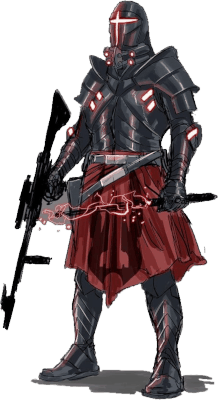
\includegraphics[width=1.2\linewidth]{_img/bestiary/citadel-guard.png}
    \vspace{-1\baselineskip} 
\end{wrapfigure}

A leur arrivé dans le périmêtre de Ktath’Atn, les héros et leur vaisseau sont dirigés vers une plateforme d’atterrissage où ils sont attendu par 4 \nameref{sec:citadel-guard} pour être escorté vers leurs quartiers avant la réception de ce soir.

L’un des gardes demande l’invitation, \nameref{sec:aphra} lui tend le document et les gardes font signe de les suivres. Ils encadre le groupe ne laissant que peu de marge de manœuvre aux héros.

Les quartiers des invités se situent dans les premiers étages de la tour. Ce sont des appartements luxueux avec largement assez de place pour que chaque membre du groupe est de quoi poser ses affaires.

Le soir tombe sur la citadelle. Laissez les héros faire ce qu’ils souhaitent pour se préparer à la réception. Les blasters et les lames ne seront pas autorisés durant la soirée, une tenue correcte est de rigueur sous peine de perdre \textbf{-2 Cha}risme. 

\subsection{La réception}

Les héros débarquent dans une salle immense, style cathédrale, très haut de plafond, colonnes, ... 

A l’intérieur une centaine de personnes, de toutes espèce et de tous genre. Certains humanoïde, d’autres d’aspect gélatineux, mais tous organiques. Des droïdes font le service au milieu des invités. 

\begin{paperbox}{Mission bonus}
Pour inciter les joueurs à interragir avec les autres invités, \nameref{sec:aphra} peut leur demander de se dispersé et de tenter d’obtenir des informations sur ce que les autres invités comptent présenter à la reine, l’objectif étant de maximiser les chances du groupe d’avoir la faveur de la \nameref{sec:ktath-atn-queen}.

Au MJ d’échanger avec les joueurs sachant que de toutes façons, la reine les choisira. 

Ce passage n’est pas obligatoire, si vos joueurs sont plus porté sur la castagne, ou si vous n’êtes pas un MJ aguerri à l’improvisation, ne vous lancez pas là dedans.
\end{paperbox}

Quand le MJ décide qu’il est temps (les joueurs n’intéragissent pas/plus) c’est le moment de faire entrer la reine et ses sbires.\\

\noindent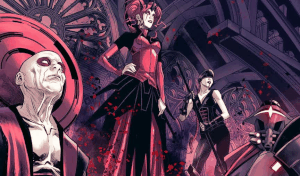
\includegraphics[width=\linewidth]{_img/places/queen-with-minions.png}

\begin{quotebox}
Bonsoir et merci à vous mes chers amis d’être venu ce soir, il me tarde de voir ce que vous avez à me présenter. Et comme promis celui qui me présentera la forme de vie organique la plus "intéressante" se vera accorder une de mes faveurs.

Mais ne trainons plus, commençons les présentations immédiatement.
\end{quotebox}

\nameref{sec:varroa} prend alors la parole et commence à appeler les invités un à un.

\begin{paperbox}{Présentations}
je ne décrit pas ici chaque présentation qui est faite. Je laisse au MJ le soin et l’imagination de faire passer des êtres plus ou moins étranges qui seront dignes ou non d’intéret. Quand les joueurs ont compris le principe, c’est a eux d’entrer en seine.
\end{paperbox}

\begin{quotebox}
\noindent\textbf{\nameref{sec:varroa}}: Docteur Aphra

\emph{\nameref{sec:aphra} fait signe aux héros de s’avancer avec elle.}

\noindent\textbf{\nameref{sec:varroa}}: Qu’avez vous a présenter à la reine.\\
\noindent\textbf{\nameref{sec:aphra}}: Un Jedi humain
\end{quotebox}

A ces mots un silence assourdissant se fit entendre. Un guerrier Ezarien sort de la foule et prend \nameref{sec:aphra} à partie. Il est grand, fin et possède une sorte d’exo-squelette qui le protège des coups directs.

\begin{quotebox}
C’est un blague, les Jedis ont été éradiqués, qu’est ce que cet humain va pouvoir faire contre moi !
\end{quotebox}

Et le guerrier Ezarien se jette sur le Jedi. Vu que le dernier a clairement montré ses intensions, la première attaque est pour le Jedi. L’enjeu ici est de faire une démonstration des pouvoirs à la reine. \'A la première utilisation visible des pouvoirs de Jedi, \nameref{sec:varroa} stoppe le combat. De son coté, le guerrier Ezarien n’a que ses poings.

Si par hasard le Jedi n’a pas accès à des pouvoirs visibles, laissez le se prendre quelques coups puis faites lui utiliser une \textbf{Poussée de Force} instinctive contre le guerrier. Cela suffira à impressionner la reine qui mettra fin au combat.

\begin{quotebox}
\noindent\textbf{\nameref{sec:varroa}}: La reine à choisie, tous les invités doivent partir immédiatement, la réception est terminée.

\emph{\nameref{sec:varroa} fait signe aux héros de s’avancer vers lui.}

\noindent\textbf{\nameref{sec:varroa}}: Ce soir nous vous offrons l’hospitalité. Demain vous déjeunerez avec la Reine, elle écoutera votre requête à ce moment. Aller dormir.
\end{quotebox}